\documentclass[compress, color = usenames, dvipsnames]{beamer}

% theme CentraleSupelec
\usepackage{theme/beamerthemeCS}

% liste de paquets
\usepackage[utf8]{inputenc}
\usepackage[francais]{babel}
\usepackage{xstring}
\usepackage{tikz}
\usetikzlibrary{shapes.arrows,chains,fit, calc,positioning, intersections}
\usepackage{pgfplots}
\usepackage{hyperref}
\usepackage{listings}
\usepackage{verbatim}
\usepackage{hyperref}
\usepackage{multimedia}
\usepackage{ifthen}

\usepackage{xcolor}% http://ctan.org/pkg/xcolor
\usepackage{colortbl}

\usepackage{pifont}
\usepackage{textcomp}
\usepackage{textpos}

\usepackage{soul}
%\usepackage{algorithmic}
\usepackage{algpseudocode}



% première page
\title[Jeu de Go \\ et \\ Exploration d'Arbre par Bandit]{Jeu de Go \\ et \\ Exploration d'Arbre par Bandit}
\subtitle[]{}
\date[]{}
\institute[]{\large CentraleSupélec -- Gif}


\begin{document}

\frame{
  \titlepage
}

\frame{
  \frametitle{IA et Jeu de Go}

  \begin{center}
  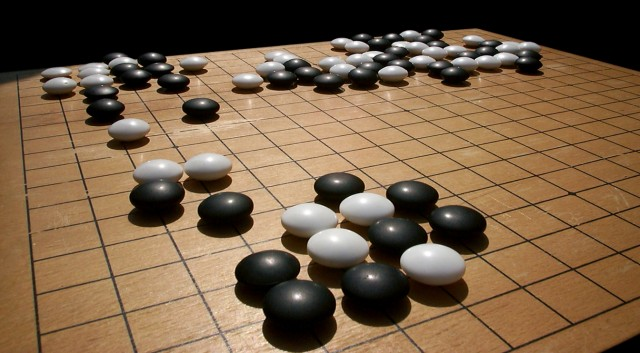
\includegraphics[width=0.8\textwidth]{figs/go-intro.jpg}
  \end{center}

}




\section{L'IA et le Jeu de Go}


\subsection{Pourquoi une IA pour le Jeu de Go?}

\frame{
  \frametitle{Pourquoi une IA pour un jeu?}

  \begin{center}
  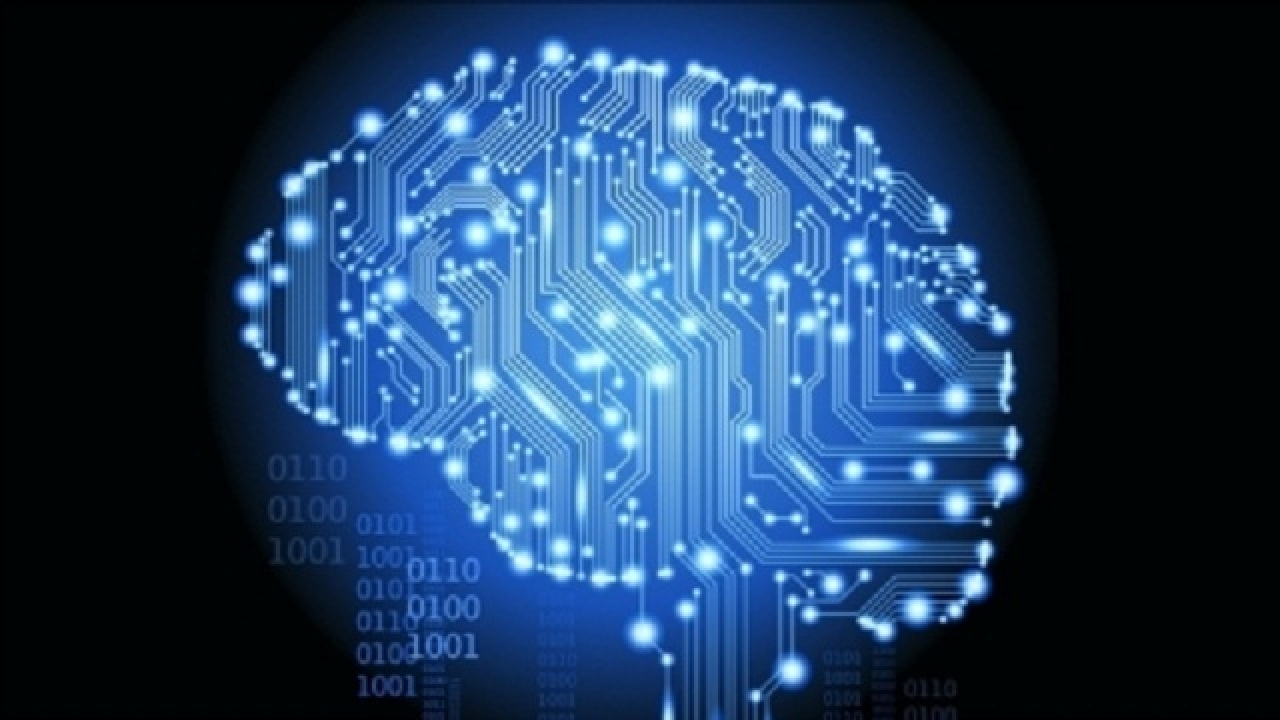
\includegraphics[width=0.5\textwidth]{figs/aigame.jpg}
  \end{center}
  \begin{itemize}
      \item Avoir une IA pour un jeu...
      \item Représentation des \red{problèmes de décision}
      \item \textbf{Environnement} bien défini: règles du jeu
      \item \textbf{Évaluation} facile: score
      \item \red{Challenge} de battre les humains
  \end{itemize}


}

\frame{
  \frametitle{Pourquoi le jeu de Go?}

  \begin{center}
  \includegraphics[width=0.5\textwidth]{figs/badukia.jpg}
  \end{center}

  \begin{itemize}
      \item un jeu de plateau qui a longtemps résisté aux IA
      \item règles \textbf{simples}
      \item méthodes classiques (alphabeta) inefficaces
  \end{itemize}

}


\subsection{Le Jeu de Go}

\frame{
  \frametitle{Histoire}

  \begin{columns}
      \begin{column}{0.3\textwidth}
          \begin{center}
              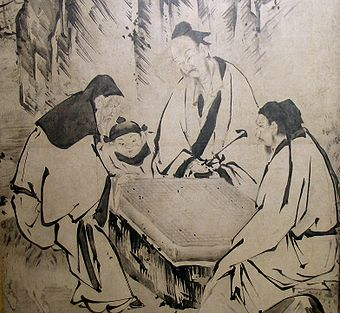
\includegraphics[width=1\textwidth]{figs/gohistory.jpg}
          \end{center}
      \end{column}
      \begin{column}{0.7\textwidth} 
          \begin{itemize}
              \item aurait été inventé en chine en 2000 BC
              \item premiers écrits: 500 BC
              \item fait parti des 4 arts majeurs chinois: peinture, calligraphie, guqin, \textit{go}
              \item se répand en Asie dès 800 dans la noblesse
              \item aujourd'hui, environ 20 millions de joueurs
          \end{itemize}
      \end{column}
  \end{columns}


}

\frame{
  \frametitle{Matériel}

  \begin{columns}
      \begin{column}{0.6\textwidth}
          \begin{itemize}
              \item plateau de jeu: Goban
              \item deux tailles 9x9 ou 19x19
              \item pierres noires et blanches 
          \end{itemize}
      \end{column}
      \begin{column}{0.4\textwidth} 
          \begin{center}
              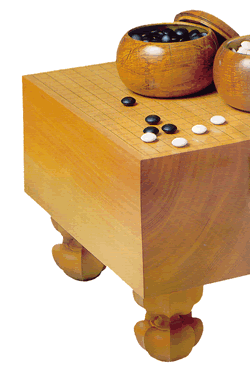
\includegraphics[width=1\textwidth]{figs/gomatos.png}
          \end{center}
      \end{column}
  \end{columns}



}

\frame{
  \frametitle{Règles: placement}

  Chaque joueur pose une pierre à tour de rôle
  Pierres posées sur les intersections
  Blanc commence

}

\frame{
  \frametitle{Règles: chaînes et capture}

  pierres reliées horizontalement ou verticalement forment une chaine
  emplacement libre autour d'une chaine: liberté
  enlever la dernière liberté d'une chaine: capture

}

\frame{
  \frametitle{Règles: fin de partie}

  les deux joueurs passent
  score

}

\frame{
  \frametitle{Règles: le ko}

  \begin{center}
  %\includegraphics[width=0.8\textwidth]{figs/goko.gif}
  \end{center}
  illustration
  histoire
  règle humain/ordinateur

}

\frame{
  \frametitle{Echelle de niveau}

}

\section{Avant l'Exploration d'Arbre par Bandit}

\frame{
  \frametitle{Présentation}

}

\frame{
  \frametitle{Alpha beta}

}

\frame{
  \frametitle{Découpage du plateau}

}

\frame{
  \frametitle{Règles expertes}

}

\frame{
  \frametitle{Échelle de niveau}

}

\section{Exploration d'Arbre par Bandit}

\subsection{Construction de l'Arbre}


\subsection{Problème de Bandit}

\begin{frame}
    \frametitle{Introduction du problème}
    \begin{center}
        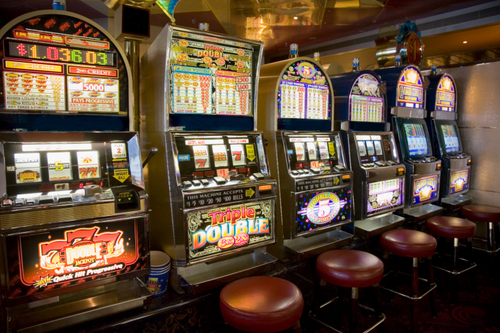
\includegraphics[scale=0.8]{figs/bandit_casino.jpg}
    \end{center}
    Dans un casino, il y a plusieurs machines à sous différentes en terme de récompense.
    \begin{itemize}
        \item Comment répartir mes pièces entre les machines?
    \end{itemize}
\end{frame}

\begin{frame}
    \frametitle{Autres problèmes similaires}
    \begin{center}
        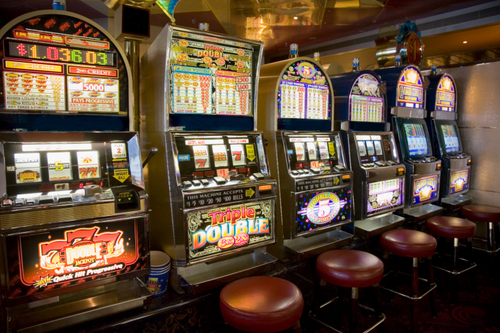
\includegraphics[scale=0.8]{figs/bandit_casino.jpg}
    \end{center}
    \begin{itemize}
        \item Essais cliniques: trouver le traitement qui fonctionne le mieux.
        \item Sélection d'un serveur dans un réseau: trouver le serveur avec le temps de réponse le plus faible.
        \item Publicité ciblée: trouver le type de pub qui intéressera le plus un utilisateur.
        \item ...
    \end{itemize}
    Ce sont des problèmes où on a plusieurs fois le même choix à effectuer. Le choix conduit à une récompense aléatoire.
\end{frame}


\begin{frame}
    \frametitle{Définition formelle}
    \begin{center}
        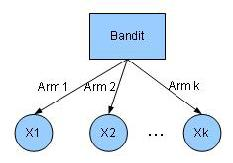
\includegraphics[scale=0.5]{figs/bandit.jpg}
    \end{center}
    \begin{itemize}
        \item un ensemble de bras $A=\{1,...,K\}$.
        \item chaque bras est associé à une distribution de probabilité $X_k$ d'espérance $\mu_k$.
        \item l'algorithme choisit un bras $a$ à chaque pas de temps.
        \item le bandit retourne une récompense $r$ : une réalisation de $X_a$.
        \item les tirages successifs sur un même bras sont indépendant et identiquement distribués.
    \end{itemize}
\end{frame}



\begin{frame}
    \frametitle{Notations supplémentaires}
    \begin{itemize}
        \item $T_i(n)$: le nombre de fois que le bras $i$ a été sélectionné au pas de temps $n$.
        \item $\mu^* = \max_{1 \le i \le K}\mu_i$
        \item $\Delta_i = \mu^* - \mu_i$ 
        \item $\Delta = \min_{i:\Delta_i > 0}\Delta_i$
    \end{itemize}


\end{frame}


\begin{frame}
    \frametitle{Objectif}

    Le but est d'optimiser le regret $R_n$ défini comme suit:

    $$R_n=\mu^*n - \mathbb{E} \sum_{j=1}^{K}  T_j(n) \mu_j$$
    $$R_n=\sum_{j=1}^{K} \Delta_j \mathbb{E} [T_j(n)]$$

\end{frame}



\begin{frame}
    \frametitle{Borne inférieure}


    Pour toute stratégie d'allocation et pour tout bras non optimal:
    $$\mathbb{E} [T_j(n)] \ge \frac{\log n}{D(p_j || p^*)}$$

    $$\mbox{où }D(p_j || p^*) = \int p_j \log \frac{p_j}{p^*}$$
    On en déduit que le meilleur regret atteignable est en ${\color{red} \log(n)}$.

    \hfill [Lai and Robbins, 1985]

\end{frame}



\begin{frame}
    \frametitle{UCB}
    Principe de l'algorithme:
    \begin{itemize}
        \item A partir des informations disponibles au temps $t$, on calcule la borne de confiance supérieur (UCB) correspondant à chaque bras.
        \item On choisit le bras qui a la valeur UCB la plus grande.
    \end{itemize}
    \hfill [Auer and all, 2002]
\end{frame}

\begin{frame}
    \frametitle{UCB}
    Calcul de la valeur UCB pour le bras $i$ au pas de temps $t$:
    $$ {\color{red} \hat{\mu}_{i,t-1}} + {\color{green} \sqrt{\frac{3\log(t)}{2T_i(t-1)}}} $$
    où $\hat{\mu}_{i,t-1} $ correspond à la moyenne empirique du bras $i$.
    
\end{frame}

\begin{frame}
    \frametitle{UCB}
    Borne sur le regret:
    $$ R_n \le 6*\sum_{i \ne i^*}\frac{\color{red}\log(n)}{\Delta_i} + K(\frac{\pi^2}{3}+1) $$
    
\end{frame}




\begin{frame}
    \frametitle{Descente dans l'arbre}
    La descente dans l'arbre se fait en considérant que chaque choix d'une branche est un problème de bandit.

    \begin{center}
        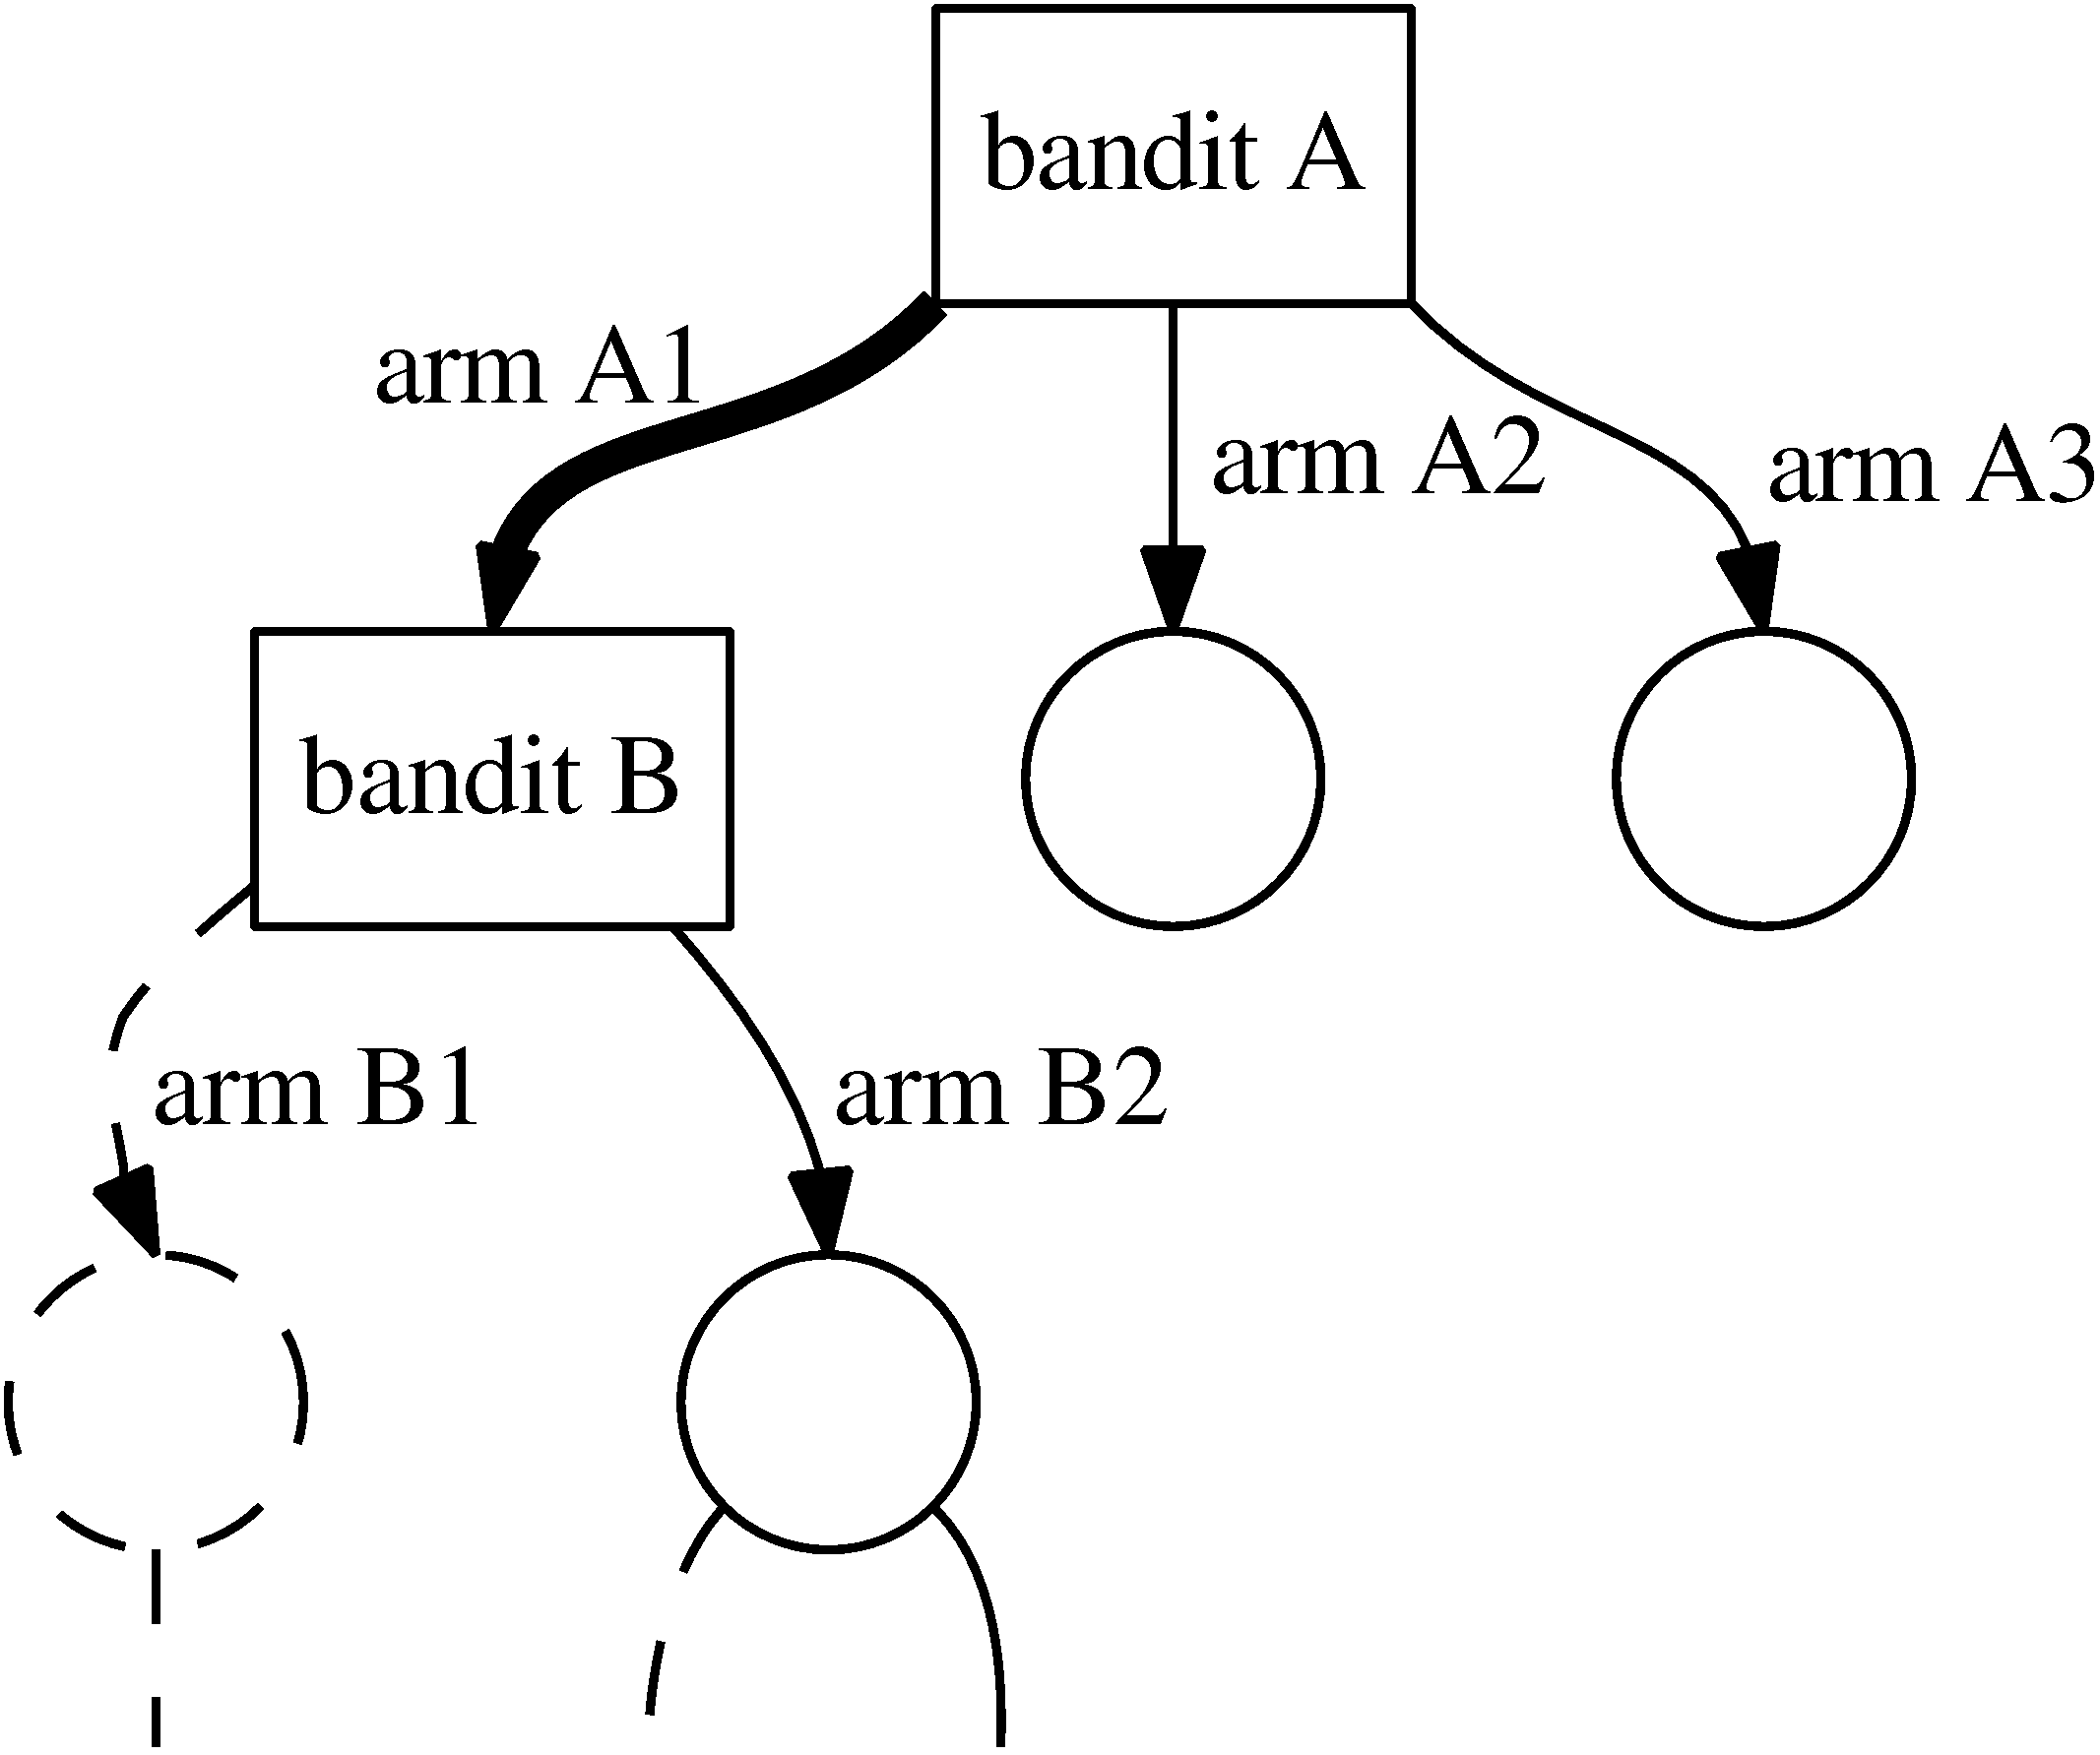
\includegraphics[scale=0.5]{figs/bandit_cascade.png}
    \end{center}


\end{frame}

\begin{frame}
    \frametitle{UCB en pratique}
    \begin{itemize}
        \item Ajout d'un paramètre $p$ de contrôle de l'exploration:
            $$ \hat{\mu}_{i,t-1} + {\color{blue}p} \sqrt{\frac{\log(t)}{T_i(t-1)}} $$
        \item Ajout de connaissances a priori $C_i(t)$:
            $$ \hat{\mu}_{i,t-1} + p \sqrt{\frac{\log(t)}{T_i(t-1)}} + {\color{blue} C_i(t)} $$
    \end{itemize}
    
\end{frame}


\subsection{Amélioration de l'Algorithme}

\frame{
  \frametitle{AMAF}

}

\frame{
  \frametitle{Ajout de Connaissances Expertes}

}

\section{Aller plus loin}

\frame{
  \frametitle{Deep Learning}

}

\frame{
  \frametitle{Autres applications}

}

\frame{
  \frametitle{Conclusion}

}





\frame{
  \frametitle{Exemple borne}

\centering

\begin{tikzpicture}

    \node [circle,draw] (a) at (0,0) {a};
    \node [circle,draw] (b) at (3,0) {b};
    \node [circle,draw] (c) at (6,0) {c};
    \node [circle,draw] (d) at (0,-4) {d};
    \node [circle,draw] (e) at (-3,-4) {e};

    \draw [dashed] (a) -- (b) node [pos=0.5]{\textbf{3}};
    \draw [dashed] (a) -- (d) node [pos=0.3]{\textbf{4}};
    \draw [dashed] (a) -- (e) node [pos=0.5]{\textbf{5}};
  
    \draw [dashed] (b) -- (c) node [pos=0.5]{\textbf{3}};
    \draw [dashed] (b) -- (d) node [pos=0.3]{5};
    \draw [dashed] (b) -- (e) node [pos=0.3]{7};
  
    \draw [dashed] (c) -- (d) node [pos=0.5]{\textbf{7}};
    \draw [dashed] (c) -- (e) node [pos=0.3]{10};
  
    \draw [dashed] (d) -- (e) node [pos=0.5]{\textbf{3}};
\end{tikzpicture}

    \begin{block}{Calcul de la borne}
        trajet déjà effectué = $\emptyset$

        $(\underbrace{3+4}_{a}+\underbrace{3+3}_{b}+\underbrace{3+7}_{c}+\underbrace{3+4}_{d}+\underbrace{3+5}_{e})/2=19$
    \end{block}

}


\end{document}
